%%%%%%%%%%%%%%%%%%%%%%%%%%%%%%%%%%%%%%%%%%%%%%%%%%%%%%%%%% 
\chapter{遷移問題への拡張} \label{chap:trans}
%%%%%%%%%%%%%%%%%%%%%%%%%%%%%%%%%%%%%%%%%%%%%%%%%%%%%%%%%%

本章では,配電網問題を遷移問題として解くことを想定し,
根付き全域森を遷移問題に拡張する手法について説明する.
また,簡単な実行例も示す.

\section{遷移問題の概要}
配電網問題を遷移問題へ拡張することで,障害時の復旧予測や,
現在の電力網構成から目的の構成へ切り替えるための手順探索などに応用できる.
しかし,スイッチの開閉を切り替える際に電力の供給が停止してしまうことを
可能な限り防ぐ必要がある.また,一度に多くのスイッチを切り替えることは
困難であると考えられる.そのため,本研究では,初期の配電網構成から,
トポロジ制約を満たした上で,一度に切り替えられるスイッチの個数に制限を設けて,
目的の配電網構成を得る遷移問題を想定した根付き全域森探索問題の拡張を行う.

根付き全域森の遷移問題への拡張について,新たに\textbf{初期状態}と\textbf{目的状態}を定義する.
初期状態と目的状態は,それぞれ対象となるグラフの根付き全域森の1つの解である.

根付き全域森の遷移問題は,入力として初期状態と目的状態が与えられ,
各ステップで根付き全域森の制約を満たしながらその状態遷移を求める問題である.
また,本研究において遷移問題が満たすべき新たな2つの制約を以下に示す.
\begin{enumerate}
 \item 初期状態から目的状態までの遷移にかかるステップ数は$t$以下である.\textbf{(ステップ数制約)}
 \item 状態が遷移する際に,変化する辺の数は$k$個以下である.\textbf{(遷移制約)}
\end{enumerate}


また,ASP言語の拡張性を利用することで,
あるステップにおいては特定の辺が使えないなどの様々な制約を
簡潔にルールとして表現することが可能であり,柔軟に追加することもできる.

\section{ASP符号化}
遷移問題に拡張した符号化\code{srf-transition}をコード\ref{code:trans}に示す.
問題の拡張にあたり,根付き全域森の符号化は\code{srf2}(コード\ref{code:srf2.lp})を基にした.
遷移問題の符号化は,全部で11個のルールで表現される.

%%%%%%%%%%%%%%%%%%%%%%%%%%%%%%%%%
\lstinputlisting[float=t,caption={%
遷移問題の論理プログラム (\code{srf-transition.lp})},%
captionpos=b,frame=single,label=code:trans,%
numbers=left,%
breaklines=true,%
columns=fullflexible,keepspaces=true,%
basicstyle=\ttfamily\scriptsize]{code/srf-transition.lp}
%%%%%%%%%%%%%%%%%%%%%%%%%%%%%%%%%

2~4行目は定数であり,定数\code{t}はステップ数制約の最大ステップ数を表す.
定数\code{k}は遷移制約において,最大で変化することのできる辺の数を表す.
4行目のファクト\code{t(0..t).}は,0から\code{t}までの各ステップ数を定義している.

7行目と10行目は,初期状態と目的状態に関する制約である.
アトム\code{init_Forest(X,Y)}は,初期状態での根付き全域森を意味する.
アトム\code{goal_Forest(X,Y)}は,目的状態での根付き全域森を意味する.
7行目のルールは,\!「\!初期状態と0ステップ目の根付き全域森は一致する」という制約を表している.
10行目のルールは,\!「\!最終状態と\code{t}ステップ目の根付き全域森は一致する」という制約を表している.
この10行目の制約を満たすことで,遷移問題のステップ数制約も満たすことを意味する.

13,16~18,21,24行目は\ref{chap:prop}章で説明した各ルールに,
ステップ数を意味する項\code{T}を導入し,各ステップにおいて各アトムが成り立つように拡張する.
これにより,各ステップにおける根付き全域森の制約を表している.

27~29行目は遷移制約を表すためのルールである.
アトム\code{dist(X,Y,T)}は,\code{T}ステップ目で辺\code{edge(X,Y)}が変化したことを意味する.
27行目のルールは,\!「\!\code{T>0}となる各ステップについて,\code{T-1}ステップ目で
森に含まれていない辺が,\code{T}ステップ目で含まれているならば,変化した辺である」
という制約を表している.
28行目のルールは,逆に\ 「\!\code{T>0}となる各ステップについて,\code{T-1}ステップ目で
森に含まれている辺が,\code{T}ステップ目で含まれていないならば,変化した辺である」
という制約を表している.
29行目のルールは,\!「\!各ステップについて,変化した辺の数は\code{k}以下となる」
という遷移制約を表している.個数制約を使うことで\code{T}ステップ目のアトム\code{dist(X,Y,T)}の数が
\code{k}以下になることを意味する.


\section{実行例}
入力として与える初期状態を図\ref{fig:init}に,目的状態を図\ref{fig:goal}にそれぞれ示す.
また,ASPファクト形式で表したものをコード\ref{code:graph-trans}に示す.
\newline

%%%%%%%%%%%%%%%%%%%%%%%%%%%%%%%%%
\begin{figure}[htbp]
 %
 \begin{minipage}{0.4\hsize}
  \centering
  %%%%%%%%%%%%%%%%%%%%%%%%%%%%%%%%%%%%%%%%%%%%%%%%%%
% 初期状態 (第6章で使う)
%%%%%%%%%%%%%%%%%%%%%%%%%%%%%%%%%%%%%%%%%%%%%%%%%%

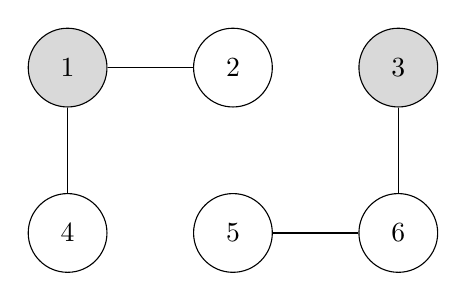
\begin{tikzpicture}[x=1.5cm,y=1.5cm,scale=0.7]

 % 設定
 \tikzset{root/.style={circle,draw=black,fill=gray!30,minimum size=1cm}}
 \tikzset{node/.style={circle,draw=black,minimum size=1cm}}
 
 % 補助線
 % \draw [help lines,blue,step=2cm] (-3,0) grid (3,-3);

 % root %
 \node[root] at (-2,0) (1){$1$};
% \node[above=0.5cm] at (1) {$r_1$};
 \node[root] at (2,0) (3){$3$};
 %\node[above=0.5cm] at (3) {$r_3$};

 % node %
 \node[node] at (0,0) (2){$2$};
 \node[node] at (-2,-2) (4){$4$};
 \node[node] at (0,-2) (5){$5$};
 \node[node] at (2,-2) (6){$6$};

 % 繋がっていない辺は破線
 %\foreach \u / \v in {2/3, 2/5, 4/5}
 %\draw [dashed] (\u) -- (\v);
 % 繋がってる辺は実線
 \foreach \u / \v in {1/2, 1/4, 3/6, 5/6}
 \draw (\u) -- (\v);

 % スイッチ switch %
 % \node at (-1,0.2) {$s_1$};
 % \node at (1,0.2) {$s_2$};
 % \node at (-2.2,-1) {$s_3$};
 % \node at (-0.2,-1) {$s_4$};
 % \node at (1.8,-1) {$s_5$};
 % \node at (-1,-1.8) {$s_6$};
 % \node at (1,-1.8) {$s_7$};
 %

\end{tikzpicture}

%%%%%%%%%%%%%%%%%%%%%%%%%%%%%%%%%%%%%%%%%%%%%%%%%%%%%%%%%%
%%% Local Variables:
%%% mode: japanese-latex
%%% TeX-master: paper.tex
%%% End:

  \caption{初期状態}
  \label{fig:init}
 \end{minipage}
 \centering
 \hspace{1cm}
 \begin{minipage}{0.4\hsize}
  \centering
  %%%%%%%%%%%%%%%%%%%%%%%%%%%%%%%%%%%%%%%%%%%%%%%%%%
% 目的状態 (第6章で使う)
%%%%%%%%%%%%%%%%%%%%%%%%%%%%%%%%%%%%%%%%%%%%%%%%%%

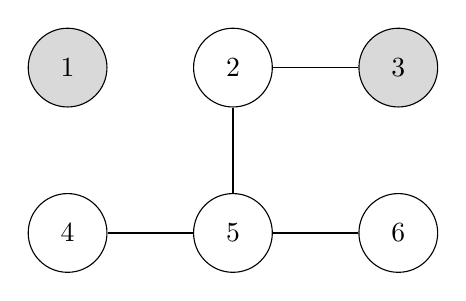
\begin{tikzpicture}[x=1.5cm,y=1.5cm,scale=0.7]

 % 設定
 \tikzset{root/.style={circle,draw=black,fill=gray!30,minimum size=1cm}}
 \tikzset{node/.style={circle,draw=black,minimum size=1cm}}
 
 % 補助線
 % \draw [help lines,blue,step=2cm] (-3,0) grid (3,-3);

 % root %
 \node[root] at (-2,0) (1){$1$};
% \node[above=0.5cm] at (1) {$r_1$};
 \node[root] at (2,0) (3){$3$};
 %\node[above=0.5cm] at (3) {$r_3$};

 % node %
 \node[node] at (0,0) (2){$2$};
 \node[node] at (-2,-2) (4){$4$};
 \node[node] at (0,-2) (5){$5$};
 \node[node] at (2,-2) (6){$6$};

 % 繋がっていない辺は破線
 %\foreach \u / \v in {2/3, 2/5, 4/5}
 %\draw [dashed] (\u) -- (\v);
 % 繋がってる辺は実線
 \foreach \u / \v in {2/3, 2/5, 4/5, 5/6}
 \draw (\u) -- (\v);

 % スイッチ switch %
 % \node at (-1,0.2) {$s_1$};
 % \node at (1,0.2) {$s_2$};
 % \node at (-2.2,-1) {$s_3$};
 % \node at (-0.2,-1) {$s_4$};
 % \node at (1.8,-1) {$s_5$};
 % \node at (-1,-1.8) {$s_6$};
 % \node at (1,-1.8) {$s_7$};
 %

\end{tikzpicture}

%%%%%%%%%%%%%%%%%%%%%%%%%%%%%%%%%%%%%%%%%%%%%%%%%%%%%%%%%%
%%% Local Variables:
%%% mode: japanese-latex
%%% TeX-master: paper.tex
%%% End:

  \caption{目的状態}
  \label{fig:goal}
 \end{minipage}
 %
\end{figure}
%%%%%%%%%%%%%%%%%%%%%%%%%%%%%%%%%
\lstinputlisting[float=t,caption={%
入力のファクト形式 (\code{graph-transition.lp})},%
captionpos=b,frame=single,label=code:graph-trans,%
numbers=left,%
breaklines=true,%
columns=fullflexible,keepspaces=true,%
basicstyle=\ttfamily\scriptsize]{code/graph-transition.lp}
%%%%%%%%%%%%%%%%%%%%%%%%%%%%%%%%%

実行例として,この入力に対してコード\ref{code:trans}の論理プログラムを
$t=3$のステップ数制約と$k=2$の遷移制約として,
{\clingo}で実行した結果をコード\ref{code:transition.log}に示す.
また,この出力をグラフ表現に変換したものを図\ref{fig:result-trans}に示す.

%%%%%%%%%%%%%%%%%%%%%%%%%%%%%%%%%
\lstinputlisting[float=t,caption={%
\code{graph-transition.lp} に対する{\clingo}の実行例}, %
captionpos=b,frame=single,label=code:transition.log,%
numbers=none,%
breaklines=true,%
columns=fullflexible,keepspaces=true,%
basicstyle=\ttfamily\scriptsize]{code/transition.log}
%%%%%%%%%%%%%%%%%%%%%%%%%%%%%%%%%

%%%%%%%%%%%%%%%%%%%%%%%%%%%%%%%%%
\begin{figure}[htbp]
 \centering
 \begin{subfigure}{0.4\hsize}
  \centering
  %%%%%%%%%%%%%%%%%%%%%%%%%%%%%%%%%%%%%%%%%%%%%%%%%%
% 実行例(t=0) (第6章で使う)
%%%%%%%%%%%%%%%%%%%%%%%%%%%%%%%%%%%%%%%%%%%%%%%%%%

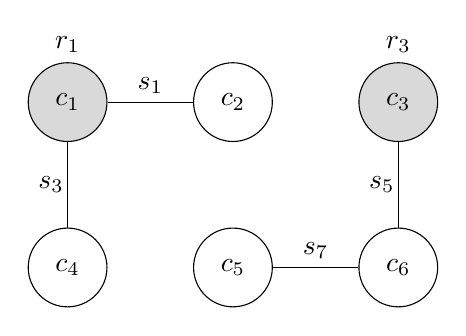
\begin{tikzpicture}[x=1.5cm,y=1.5cm,scale=0.7]

 % 設定
 \tikzset{root/.style={circle,draw=black,fill=gray!30,minimum size=1cm}}
 \tikzset{node/.style={circle,draw=black,minimum size=1cm}}
 
 % 補助線
 % \draw [help lines,blue,step=2cm] (-3,0) grid (3,-3);

 % 時間 %
 % \node[rectangle,draw=black] at (-3,1) {$t=0$};

 % root %
 \node[root] at (-2,0) (1){$c_1$};
 \node[above=0.5cm] at (1) {$r_1$};
 \node[root] at (2,0) (3){$c_3$};
 \node[above=0.5cm] at (3) {$r_3$};

 % node %
 \node[node] at (0,0) (2){$c_2$};
 \node[node] at (-2,-2) (4){$c_4$};
 \node[node] at (0,-2) (5){$c_5$};
 \node[node] at (2,-2) (6){$c_6$};

 % 繋がっていない辺は破線
 %\foreach \u / \v in {2/3, 2/5, 4/5}
 %\draw [dashed] (\u) -- (\v);
 % 繋がってる辺は実線
 \foreach \u / \v in {1/2, 1/4, 3/6, 5/6}
 \draw (\u) -- (\v);

 % スイッチ switch %
  \node at (-1,0.2) {$s_1$};
 % \node at (1,0.2) {$s_2$};
  \node at (-2.2,-1) {$s_3$};
 % \node at (-0.2,-1) {$s_4$};
  \node at (1.8,-1) {$s_5$};
 % \node at (-1,-1.8) {$s_6$};
  \node at (1,-1.8) {$s_7$};
 %

\end{tikzpicture}

%%%%%%%%%%%%%%%%%%%%%%%%%%%%%%%%%%%%%%%%%%%%%%%%%%%%%%%%%%
%%% Local Variables:
%%% mode: japanese-latex
%%% TeX-master: paper.tex
%%% End:

  \caption{$t=0$ (初期状態)}
 \end{subfigure}
 \hspace{1cm}
 \begin{subfigure}{0.4\hsize}
  \centering
  %%%%%%%%%%%%%%%%%%%%%%%%%%%%%%%%%%%%%%%%%%%%%%%%%%
% 実行例(t=1) (第6章で使う)
%%%%%%%%%%%%%%%%%%%%%%%%%%%%%%%%%%%%%%%%%%%%%%%%%%

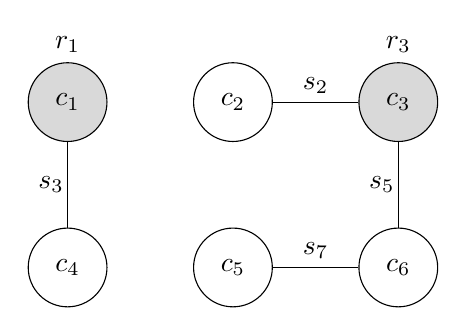
\begin{tikzpicture}[x=1.5cm,y=1.5cm,scale=0.7]

 % 設定
 \tikzset{root/.style={circle,draw=black,fill=gray!30,minimum size=1cm}}
 \tikzset{node/.style={circle,draw=black,minimum size=1cm}}
 
 % 補助線
 % \draw [help lines,blue,step=2cm] (-3,0) grid (3,-3);

 % 時間 %
 % \node[rectangle,draw=black] at (-3,1) {$t=1$};

 % root %
 \node[root] at (-2,0) (1){$c_1$};
 \node[above=0.5cm] at (1) {$r_1$};
 \node[root] at (2,0) (3){$c_3$};
 \node[above=0.5cm] at (3) {$r_3$};

 % node %
 \node[node] at (0,0) (2){$c_2$};
 \node[node] at (-2,-2) (4){$c_4$};
 \node[node] at (0,-2) (5){$c_5$};
 \node[node] at (2,-2) (6){$c_6$};

 % 繋がっていない辺は破線
 %\foreach \u / \v in {2/3, 2/5, 4/5}
 %\draw [dashed] (\u) -- (\v);
 % 繋がってる辺は実線
 \foreach \u / \v in {2/3, 1/4, 3/6, 5/6}
 \draw (\u) -- (\v);

 % スイッチ switch %
 % \node at (-1,0.2) {$s_1$};
 %
 \node at (1,0.2) {$s_2$};
 \node at (-2.2,-1) {$s_3$};
 % \node at (-0.2,-1) {$s_4$};
 \node at (1.8,-1) {$s_5$};
 % \node at (-1,-1.8) {$s_6$};
 \node at (1,-1.8) {$s_7$};
 %

\end{tikzpicture}

%%%%%%%%%%%%%%%%%%%%%%%%%%%%%%%%%%%%%%%%%%%%%%%%%%%%%%%%%%
%%% Local Variables:
%%% mode: japanese-latex
%%% TeX-master: paper.tex
%%% End:

  \caption{$t=1$}
 \end{subfigure}
 \\ \vspace{0.5cm}
 \begin{subfigure}{0.4\hsize}
  \centering
  %%%%%%%%%%%%%%%%%%%%%%%%%%%%%%%%%%%%%%%%%%%%%%%%%%
% 実行例(t=2) (第6章で使う)
%%%%%%%%%%%%%%%%%%%%%%%%%%%%%%%%%%%%%%%%%%%%%%%%%%

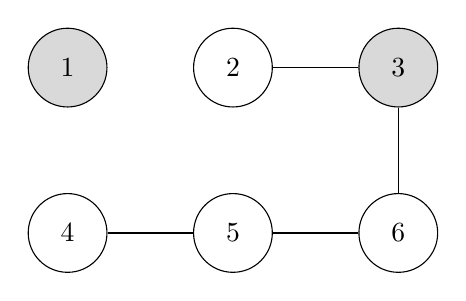
\begin{tikzpicture}[x=1.5cm,y=1.5cm,scale=0.7]

 % 設定
 \tikzset{root/.style={circle,draw=black,fill=gray!30,minimum size=1cm}}
 \tikzset{node/.style={circle,draw=black,minimum size=1cm}}
 
 % 補助線
 % \draw [help lines,blue,step=2cm] (-3,0) grid (3,-3);

 % 時間 %
 % \node[rectangle,draw=black] at (-3,1) {$t=2$};

 % root %
 \node[root] at (-2,0) (1){$1$};
% \node[above=0.5cm] at (1) {$r_1$};
 \node[root] at (2,0) (3){$3$};
 %\node[above=0.5cm] at (3) {$r_3$};

 % node %
 \node[node] at (0,0) (2){$2$};
 \node[node] at (-2,-2) (4){$4$};
 \node[node] at (0,-2) (5){$5$};
 \node[node] at (2,-2) (6){$6$};

 % 繋がっていない辺は破線
 %\foreach \u / \v in {2/3, 2/5, 4/5}
 %\draw [dashed] (\u) -- (\v);
 % 繋がってる辺は実線
 \foreach \u / \v in {2/3, 4/5, 3/6, 5/6}
 \draw (\u) -- (\v);

 % スイッチ switch %
 % \node at (-1,0.2) {$s_1$};
 % \node at (1,0.2) {$s_2$};
 % \node at (-2.2,-1) {$s_3$};
 % \node at (-0.2,-1) {$s_4$};
 % \node at (1.8,-1) {$s_5$};
 % \node at (-1,-1.8) {$s_6$};
 % \node at (1,-1.8) {$s_7$};
 %

\end{tikzpicture}

%%%%%%%%%%%%%%%%%%%%%%%%%%%%%%%%%%%%%%%%%%%%%%%%%%%%%%%%%%
%%% Local Variables:
%%% mode: japanese-latex
%%% TeX-master: paper.tex
%%% End:

  \caption{$t=2$}
 \end{subfigure}
 \hspace{1cm}
 \begin{subfigure}{0.4\hsize}
  \centering
  %%%%%%%%%%%%%%%%%%%%%%%%%%%%%%%%%%%%%%%%%%%%%%%%%%
% 実行例(t=3) (第6章で使う)
%%%%%%%%%%%%%%%%%%%%%%%%%%%%%%%%%%%%%%%%%%%%%%%%%%
\begin{tikzpicture}[scale=0.6]

 % 設定
 \tikzset{node/.style={circle,draw=black,fill=white}}

 \definecolor{edge1}{RGB}{191,0,0}
 \definecolor{node1}{RGB}{249,200,200}
 \definecolor{edge3}{RGB}{38,38,134}
 \definecolor{node3}{RGB}{200,200,249}

 % 補助線
 % \draw [help lines,blue] (0,0) grid (20,6);

 % node %
 \node[circle, ultra thick, draw=edge1, fill=node1](out1){1};
 \node[node, fill=node3, right=of out1] (out2){2};
 \node[circle, ultra thick, draw=edge3,fill=node3, right=of out2](out3){3};
 \node[node, fill=node3, below=of out1] (out4){4};
 \node[node, fill=node3, below=of out2] (out5){5};
 \node[node, fill=node3, below=of out3] (out6){6};

 \foreach \u / \v in {}
 \draw [very thick, edge1] (\u) -- (\v);

 \foreach \u / \v in {out2/out3,out2/out5,out4/out5,out5/out6}
 \draw [very thick, edge3](\u) -- (\v);
\end{tikzpicture}

%%%%%%%%%%%%%%%%%%%%%%%%%%%%%%%%%%%%%%%%%%%%%%%%%%%%%%%%%%
%%% Local Variables:
%%% mode: japanese-latex
%%% TeX-master: paper.tex
%%% End:

  \caption{$t=3$ (目的状態)}
 \end{subfigure}
 %
 \caption{実行例(コード\ref{code:transition.log})のグラフ表現}
 \label{fig:result-trans}
\end{figure}
%%%%%%%%%%%%%%%%%%%%%%%%%%%%%%%%%


%%% Local Variables:
%%% mode: japanese-latex
%%% TeX-master: "paper"
%%% End:
